
% =============================================================================
\section{Evaluation}
\label{sev:eval}



\begin{figure*}[t]
    \centering

    \begin{minipage}{0.32\textwidth}
        \centering
        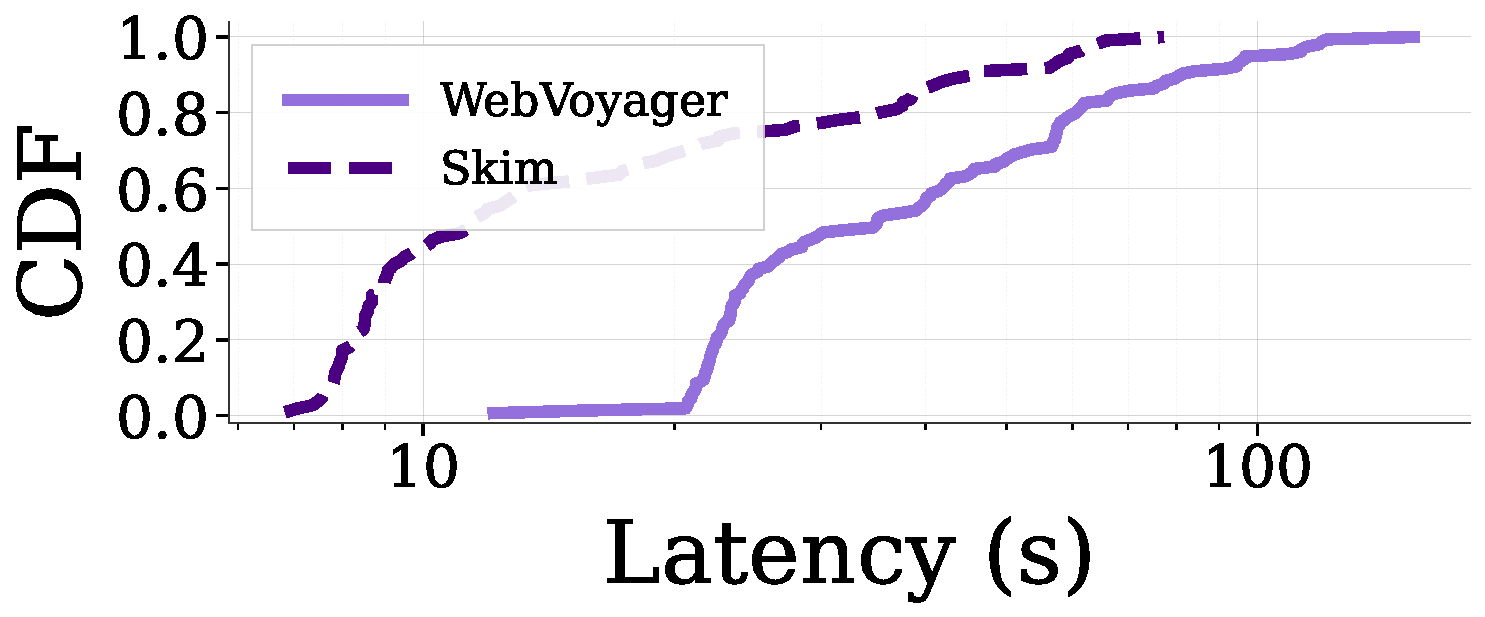
\includegraphics[width=\linewidth]{figures/latency_successful_tasks_webvoyager_evaluation_cdf.pdf}
    \end{minipage}
    \hfill
    \begin{minipage}{0.32\textwidth}
        \centering
        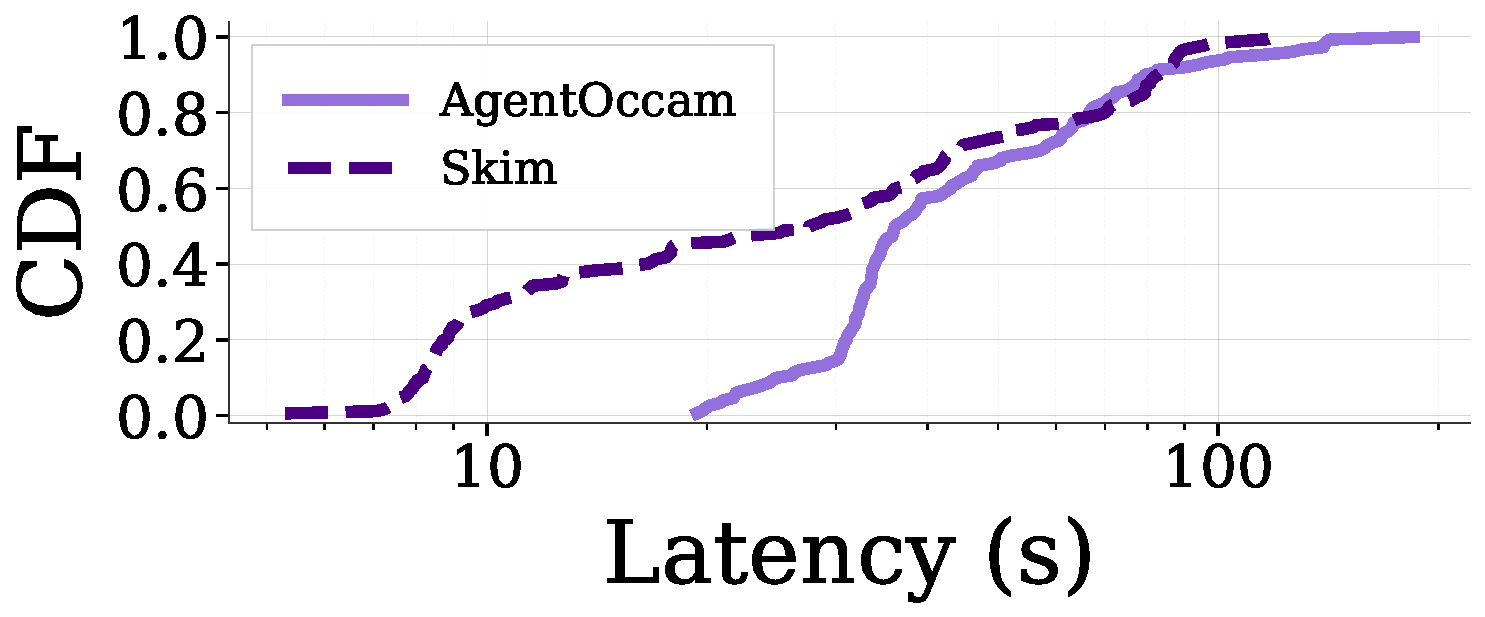
\includegraphics[width=\linewidth]{figures/latency_successful_tasks_agentoccam_evaluation_cdf.pdf}
    \end{minipage}
    \hfill
    \begin{minipage}{0.32\textwidth}
        \centering
        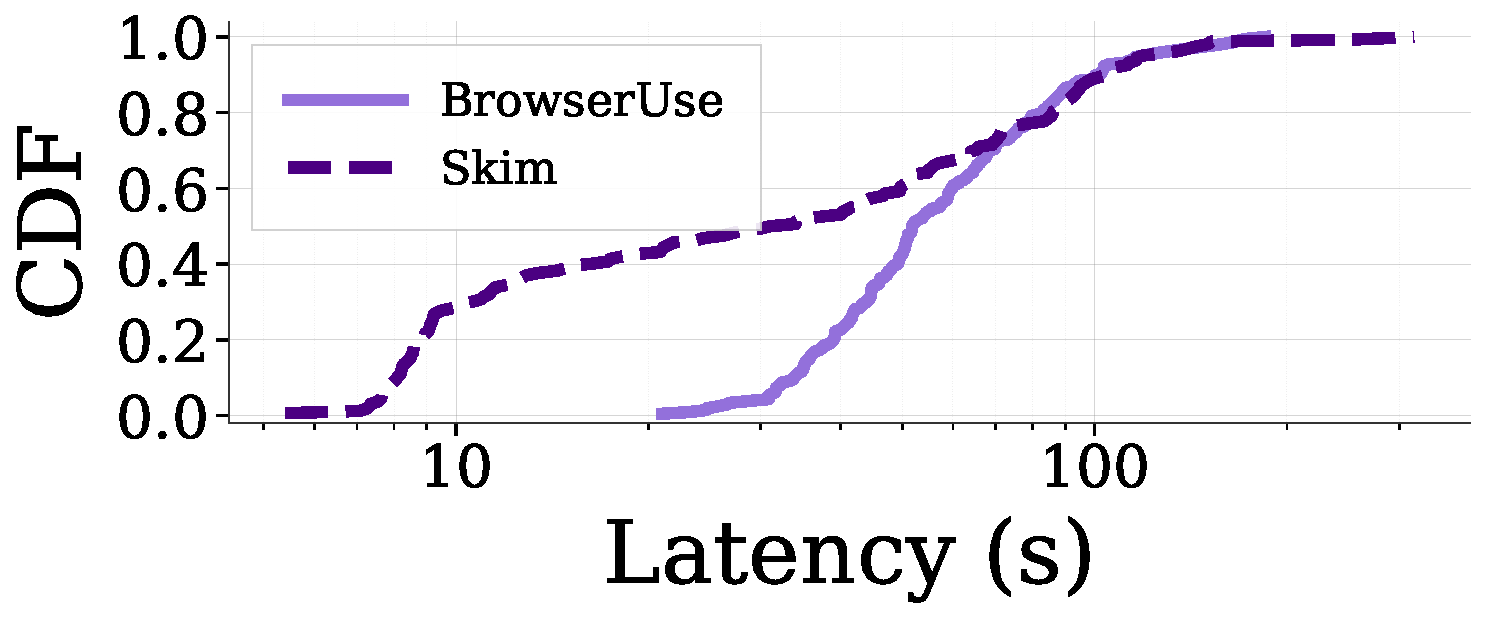
\includegraphics[width=\linewidth]{figures/latency_successful_tasks_browseruse_evaluation_cdf.pdf}
    \end{minipage}

    \tightcaption{End-to-end task latencies for WebVoyager (left), AgentOccam (middle), and BrowserUse (right) across all tasks.}
    \label{fig:end-to-end-latencies}
\end{figure*}
\begin{figure*}[t]
    \centering

    \begin{minipage}{0.32\textwidth}
        \centering
        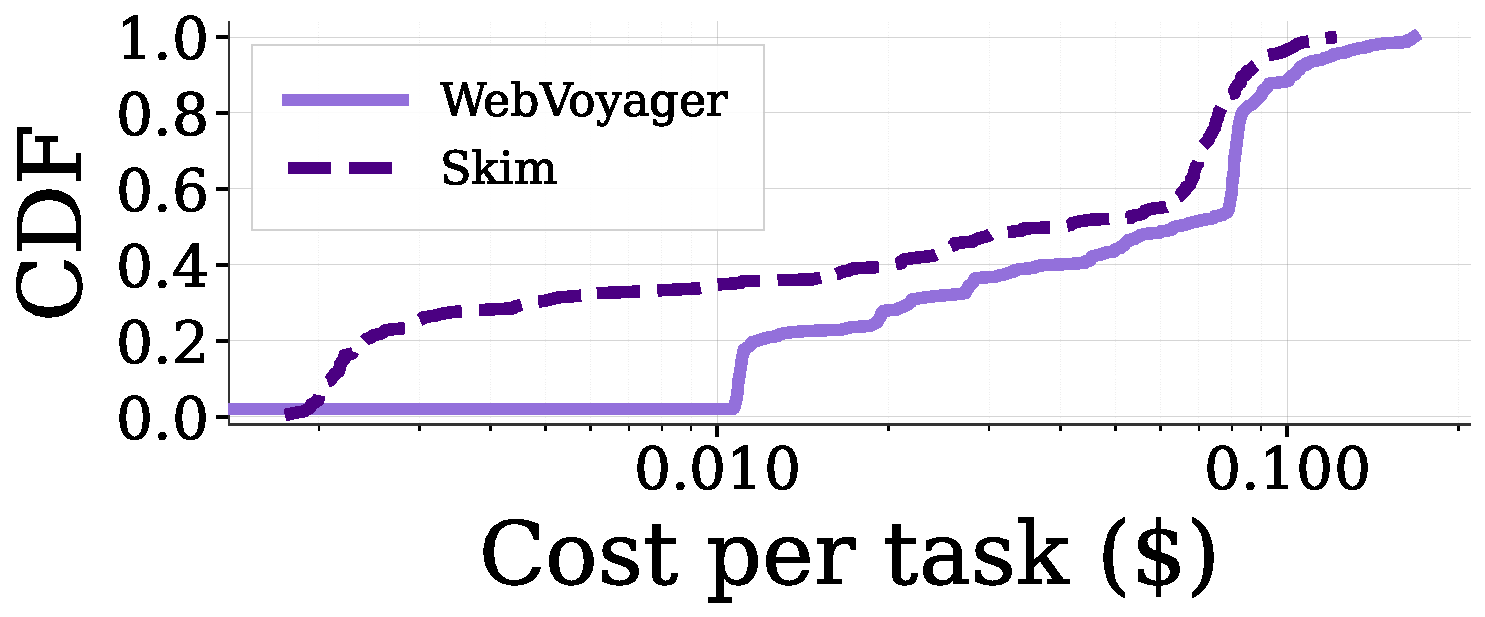
\includegraphics[width=\linewidth]{figures/monetary_costs_webvoyager_evaluation_cdf.pdf}
    \end{minipage}
    \hfill
    \begin{minipage}{0.32\textwidth}
        \centering
        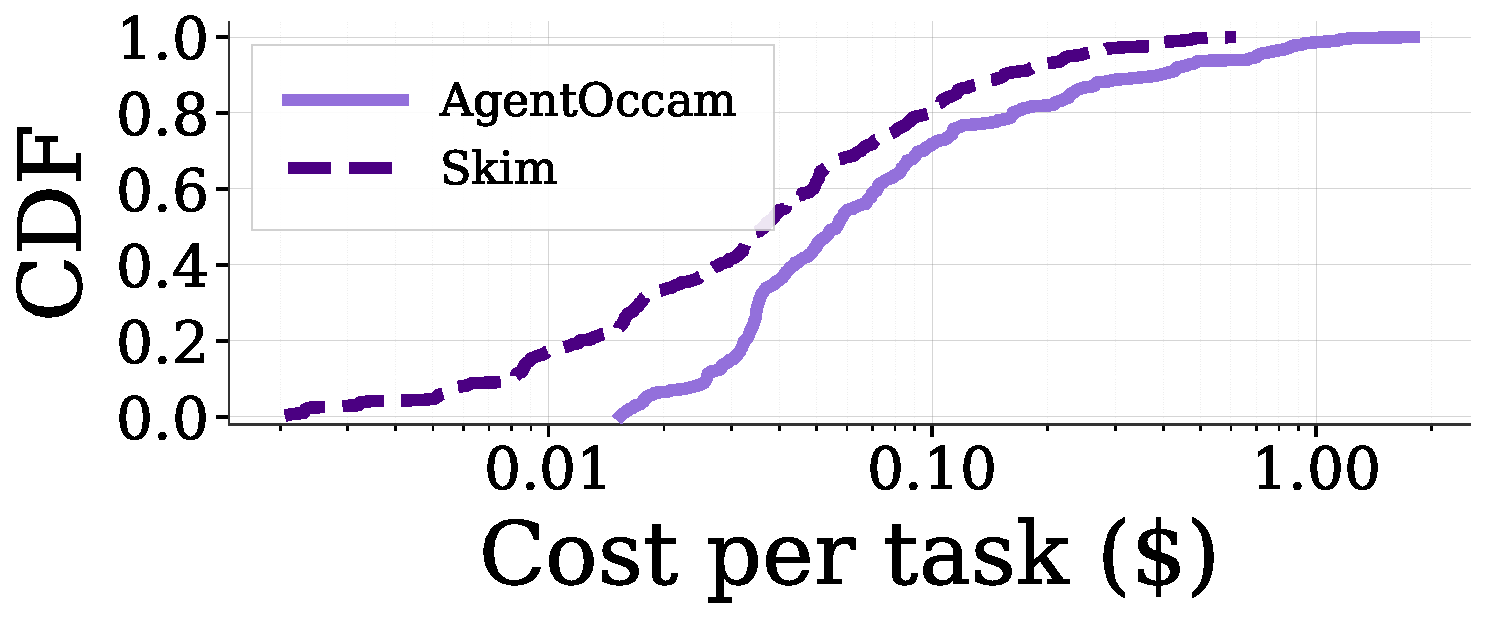
\includegraphics[width=\linewidth]{figures/monetary_costs_agentoccam_evaluation_cdf.pdf}
    \end{minipage}
    \hfill
    \begin{minipage}{0.32\textwidth}
        \centering
        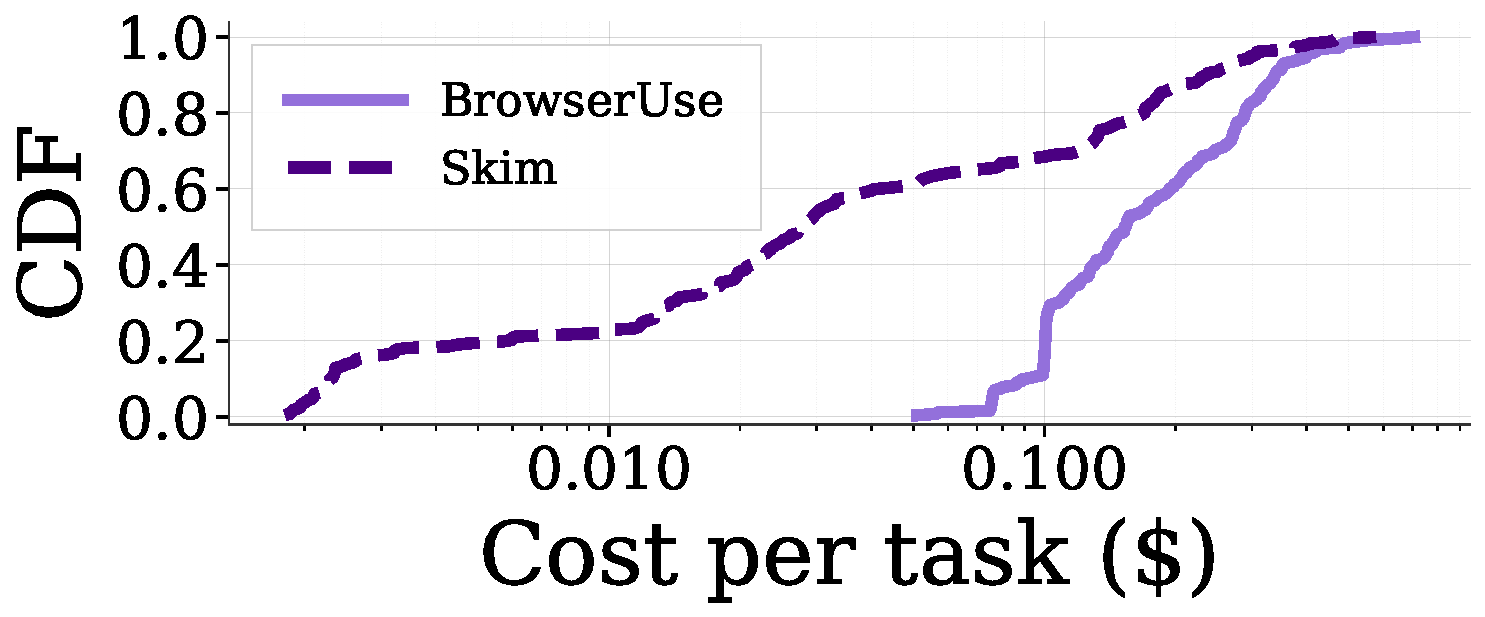
\includegraphics[width=\linewidth]{figures/monetary_costs_browseruse_evaluation_cdf.pdf}
    \end{minipage}

    \tightcaption{End-to-end task costs for WebVoyager (left), AgentOccam (middle), and BrowserUse (right) across all tasks.}
    \label{fig:end-to-end-costs}
\end{figure*}



\subsection{Methodology}
\begin{sloppypar}
We evaluate \sys atop three representative ReAct-based web agents: WebVoyager~\cite{webvoyager}, AgentOccam~\cite{agentoccam}, and BrowserUse~\cite{browseruse}. WebVoyager is a multimodal agent over rendered screenshots, serving as a strong baseline for general-purpose live-web navigation. AgentOccam emphasizes lightweight reasoning and action efficiency through aggressive state pruning over text-based DOM observations, representing cost-conscious agent designs. BrowserUse is a production-oriented browser-automation framework that tightly couples LLM reasoning with browser-control primitives, reflecting the deployment-focused agents used in retrieval and automation pipelines. Together, these systems span a range of reasoning styles, observation modalities, and execution overheads.
\end{sloppypar}

We consider two representative benchmarks. WebVoyager~\cite{webvoyager} spans 15 real-world websites with open-ended navigation, retrieval, and structured extraction tasks. WebShop~\cite{webshop} provides a shopping environment derived from Amazon product data, focused on multi-step product search and selection. Because evaluating live ReAct agents at scale is both computationally expensive and time-consuming (browsers and frontier models at each step), we conduct our experiments on a representative subset of 300+ tasks randomly drawn across the two benchmarks. Each task is executed on every agent backend with \sys. This scale captures a broad range of websites, task structures, and execution behaviors while keeping evaluation practically tractable. Ablations and detailed analyses are reported on AgentOccam and WebVoyager, though all trends hold for other combinations. Metrics include end-to-end latency, per-task dollar cost, and task success rate. Latency and cost are measured over complete task executions including failures and cascades.

%We evaluate \sys atop three representative ReAct-based web agents: WebVoyager, AgentOccam, and BrowserUse. WebVoyager is a canonical multimodal ReAct agent that operates over rendered webpages using iterative reasoning and browser interaction, and serves as a strong baseline for general-purpose live-web navigation. AgentOccam emphasizes lightweight reasoning and action efficiency through aggressive state pruning and simplified decision making, making it representative of cost-conscious agent designs. BrowserUse is a production-oriented browser automation framework that tightly couples LLM reasoning with browser control primitives and realistic interaction APIs, reflecting the growing class of deployment-focused web agents used in retrieval and automation pipelines. Together, these systems span a range of reasoning styles, observation modalities, and execution overheads, allowing us to evaluate whether \sys generalizes across diverse ReAct implementations rather than overfitting to a single agent architecture.


%We evaluate on two representative benchmarks: WebVoyager and WebShop. WebVoyager consists of live-web tasks spanning 15 real-world websites and exercises open-ended navigation, retrieval, and structured extraction. WebShop provides a controlled shopping environment derived from Amazon product data and focuses on multi-step product search and selection tasks. Because evaluating live ReAct agents is both computationally expensive and time-consuming (particularly in their default form using browsers and frontier models at each step), we conduct our experiments on a representative subset of 300 tasks randomly drawn across the two benchmarks. This scale is sufficient to capture a broad range of websites, task structures, and execution behaviors while keeping evaluation practically tractable.

%Metrics include end-to-end wall-clock latency, inclusive of routing, fetching, parsing, inference, verification, and cascade overhead; per-task dollar cost, including frontier API usage and local-model inference cost; and task success rate. Latency and cost are measured over complete task executions including failures and cascades.


% Ours webshop WebVoyager: 66 / 150, default: 72 / 151
% Ours WebVoyager WebVoyager 39 / 151 (upto20: 120 / 303), default: 41 / 150
%
% Ours webshop AgentOccam 83 / 150, default: 75 / 150
% Ours WebVoyager AgentOccam 73 / 151, default: 74 / 151
%
% Ours webshop browseruse 58 / 150, default: 71 / 150
% Ours WebVoyager browseruse 79 / 151, default: 64 / 151



\subsection{Main Results}

Figures~\ref{fig:end-to-end-latencies}-\ref{fig:end-to-end-costs} report per-task latency and cost CDFs against each baseline. \sys achieves its largest gains on tasks that complete on the speculative fast path: navigation collapses to direct URL synthesis, repeated frontier-model inference is avoided, and extraction runs over condensed HTML with lightweight models. These tasks complete at a small fraction of full-ReAct latency and cost. Gains diminish in the tail as tasks trigger fallback to the underlying ReAct agent, either because verification rejected the fast path or because no template matched. However, \sys often preserves partial navigational progress through warm-start URLs, so even fallbacks frequently outperform cold-start ReAct (Figures~\ref{fig:warm-start-webvoyager-savings}-\ref{fig:warm-start-agentoccam-savings}). At the far tail, performance converges to the baseline in two cases: when \sys determines that no fast path applies and routes directly to the ReAct backend, or when the speculative attempt reaches a URL without useful progress; for the latter, overhead is bound by the failed attempt and verification stage.

Despite the fallback cases, \sys preserves end-to-end accuracy within noise of full ReAct (Table~\ref{t:accuracy-comparison}) while substantially reducing median latency and cost. Two properties drive this. First, speculative execution follows trajectories grounded in real structural patterns from offline profiling -- URL templates, search behavior, pagination structure, answer schemas -- that are tied to the site's core purpose and remain stable even as underlying content changes, rather than unconstrained lightweight reasoning over arbitrary pages. Second, every fast-path result is gated through verification before commitment, catching missing fields, unexpected page structures, failed extraction, and stale templates. When verification rejects, \sys reverts to the full ReAct agent rather than committing a wrong answer, so failures degrade gracefully into standard agent behavior.
\begin{table}[t]
    \centering
    \small
    \begin{tabular}{lcc}
        \toprule
        \textbf{Agent} & \textbf{Our accuracy} & \textbf{Agent accuracy} \\
        \midrule
        WebVoyager & 40.6\% & 37.6\% \\
        AgentOccam & 52.0\% & 49.6\% \\
        BrowserUse & 45.6\% & 45.0\% \\
        \bottomrule
    \end{tabular}
    \vspace{8pt}
    \tightcaption{Accuracies for \sys and default web agents.}
        \label{t:accuracy-comparison}
\end{table}

\para{Aggregate mode.} \sys{}'s cost savings can be repurposed to run multiple speculative trials per task within the baseline's single-execution budget, with results aggregated across trajectories. For instance, on the WebVoyager benchmark with AgentOccam, this enables \sys to run an average of four additional trajectories per task, with accuracy wins varying by sampling strategy: upper-bound wins (i.e., assuming oracle selection of the best trial) reach 16.7 percentage points, while majority vote yields 4.2-percentage-point improvements. 



%On 24 tasks with five trials each, individual trials match baseline accuracy (19-21/24 per trial vs. 19/24 baseline), but aggregating lifts performance substantially: 23/24 tasks have at least one correct trial, and majority voting (≥3/5 correct) achieves 20/24. This translates to accuracy improvements of 4.2 percentage points (majority vote, 79.2\% → 83.3\%) and 16.7 percentage points (≥1 correct, 79.2\% → 95.8\%) over the baseline. The gain comes from \sys{}'s cost headroom enabling multiple trajectory explorations per task — a regime the baseline cannot afford — with verifier-based selection across trials.


\begin{comment}
Figures~\ref{fig:eval-latency-agentoccam} and
\ref{fig:eval-latency-webvoyager} report per-task latency CDFs
against each baseline. \sys achieves its largest gains on tasks
that successfully complete on the speculative fast path. In these
cases, the system bypasses the iterative ReAct loop entirely:
navigation collapses to direct URL synthesis and retrieval,
execution avoids repeated frontier-model inference, and extraction
runs over condensed HTML using lightweight models. These tasks
therefore complete with only a small fraction of the latency and
cost of full ReAct execution.

The gains diminish in the tail of the distribution as more tasks
trigger fallback to the underlying ReAct agent. Fallbacks occur
when verification rejects the speculative execution path or when
a task does not match a reusable template. Even in these cases,
however, \sys often preserves partial navigational progress through
warm-start URLs inherited from the failed fast path. As a result,
many fallback tasks still outperform cold-start ReAct execution
despite requiring full-agent recovery.

At the far tail, performance converges toward the baseline ReAct
agent. This occurs in two common cases: either \sys determines
ex ante that no reliable fast path applies and routes directly to
the ReAct backend, or the speculative trajectory reaches a URL
that provides little useful navigational progress, making recovery
behavior similar to executing the ReAct agent from scratch. In
the latter case, the additional overhead is limited to the small
cost of the failed speculative attempt and verification stage.
Importantly, despite these fallback cases, \sys preserves end-to-end
accuracy statistically within noise of full ReAct
(Figures~\ref{fig:eval-acc-webvoyager},
\ref{fig:eval-acc-webshop}) while substantially reducing median
latency and cost.

Against the capability-stripped baselines, \sys preserves the
coverage and robustness of full ReAct execution while approaching
the cost profile of lightweight retrieval pipelines on fast-path
tasks. The key reason accuracy is preserved is that speculative
execution is not based on heuristic shortcuts or approximate
trajectory guessing; it is grounded in real structural patterns
observed during offline profiling of each site. The fast path
reuses stable site conventions --- URL templates, search behavior,
pagination structure, and answer schemas --- that are tied to the
site’s core purpose and therefore remain comparatively stable over
time even as underlying content changes. As a result, speculative
execution follows trajectories that are already known to be valid
for that site rather than attempting unconstrained lightweight
reasoning over arbitrary pages.

Robust verification further prevents speculative errors from
propagating into incorrect final outputs. Every fast-path result is
validated through schema checks, content-consistency verification,
and runtime monitoring before commitment. When verification detects
that the speculative execution path may have diverged from the
task -- due to missing fields, unexpected page structure, failed
content extraction, or stale templates -- \sys automatically
reverts to the default ReAct agent. Because ReAct execution serves
as the recovery path rather than being replaced entirely, failures
of speculative execution degrade gracefully into standard agent
behavior instead of causing catastrophic task failure. In effect,
\sys preserves the accuracy envelope of full ReAct execution while
speculatively bypassing its cost whenever the site structure makes
doing so safe.
\end{comment}



\begin{figure}[t]
    \centering
    \begin{minipage}{0.48\columnwidth}
        \centering
        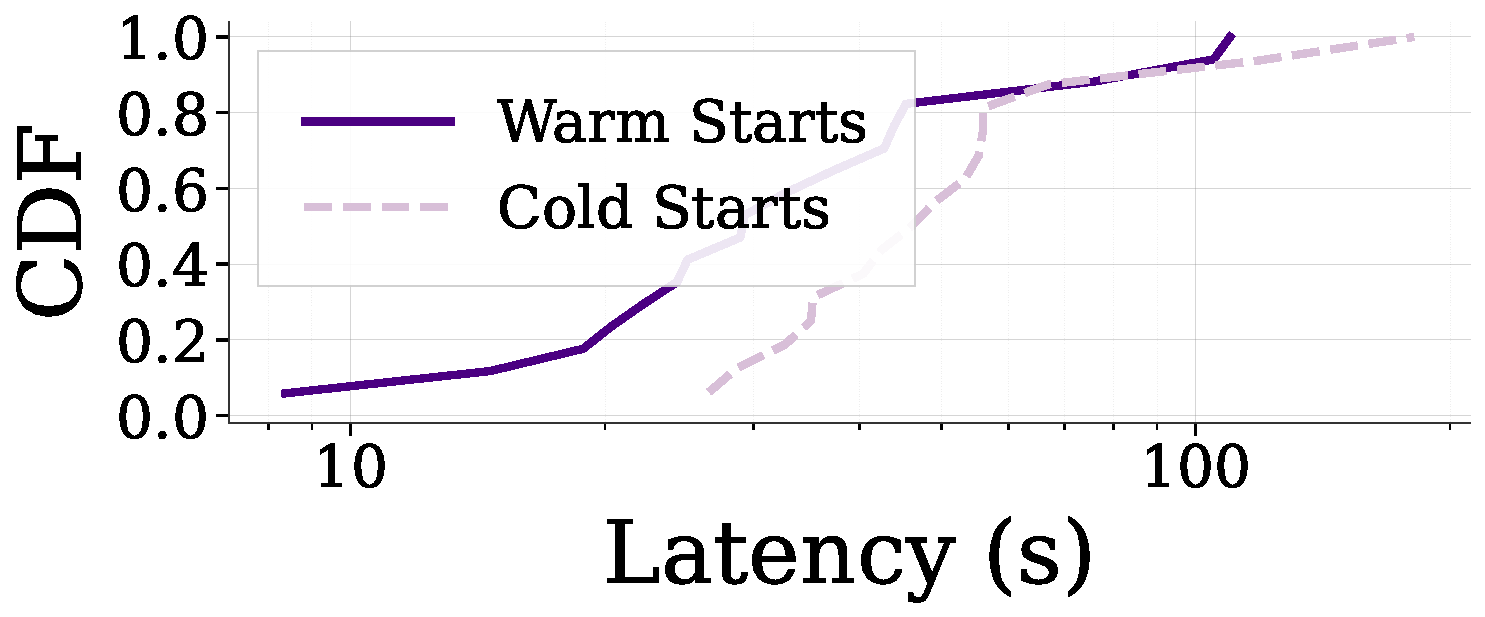
\includegraphics[width=\linewidth]{figures/latency_webvoyager_warm_cold_cdf.pdf}
        \tightcaption{Warm start savings for WebVoyager.}
        \label{fig:warm-start-webvoyager-savings}
    \end{minipage}
    \hfill
    \begin{minipage}{0.48\columnwidth}
        \centering
        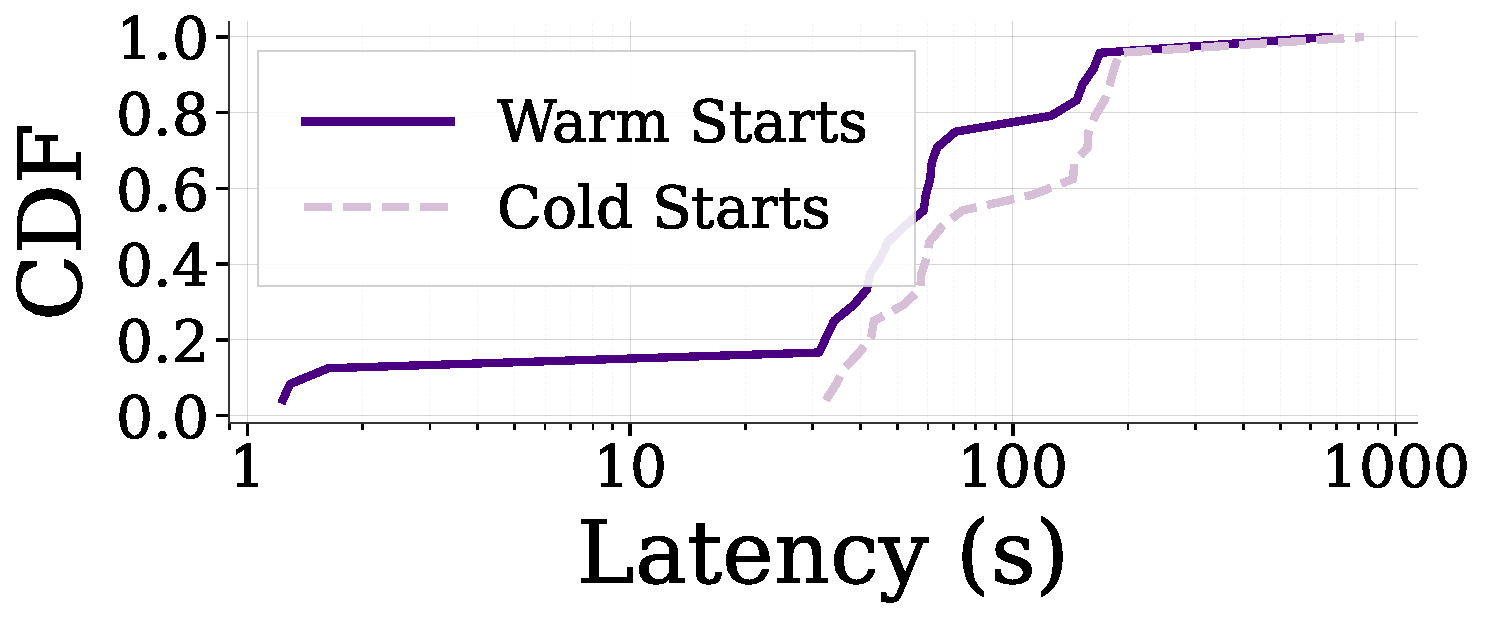
\includegraphics[width=\linewidth]{figures/latency_agentoccam_warm_cold_cdf.pdf}
        \tightcaption{Warm start savings for AgentOccam.}
        \label{fig:warm-start-agentoccam-savings}
    \end{minipage}
\end{figure}


% Results we want to get: latency of fast path vs default, Accuracy of fast path vs default
% Latencies and costs by task

\begin{figure}[t]
    \centering
    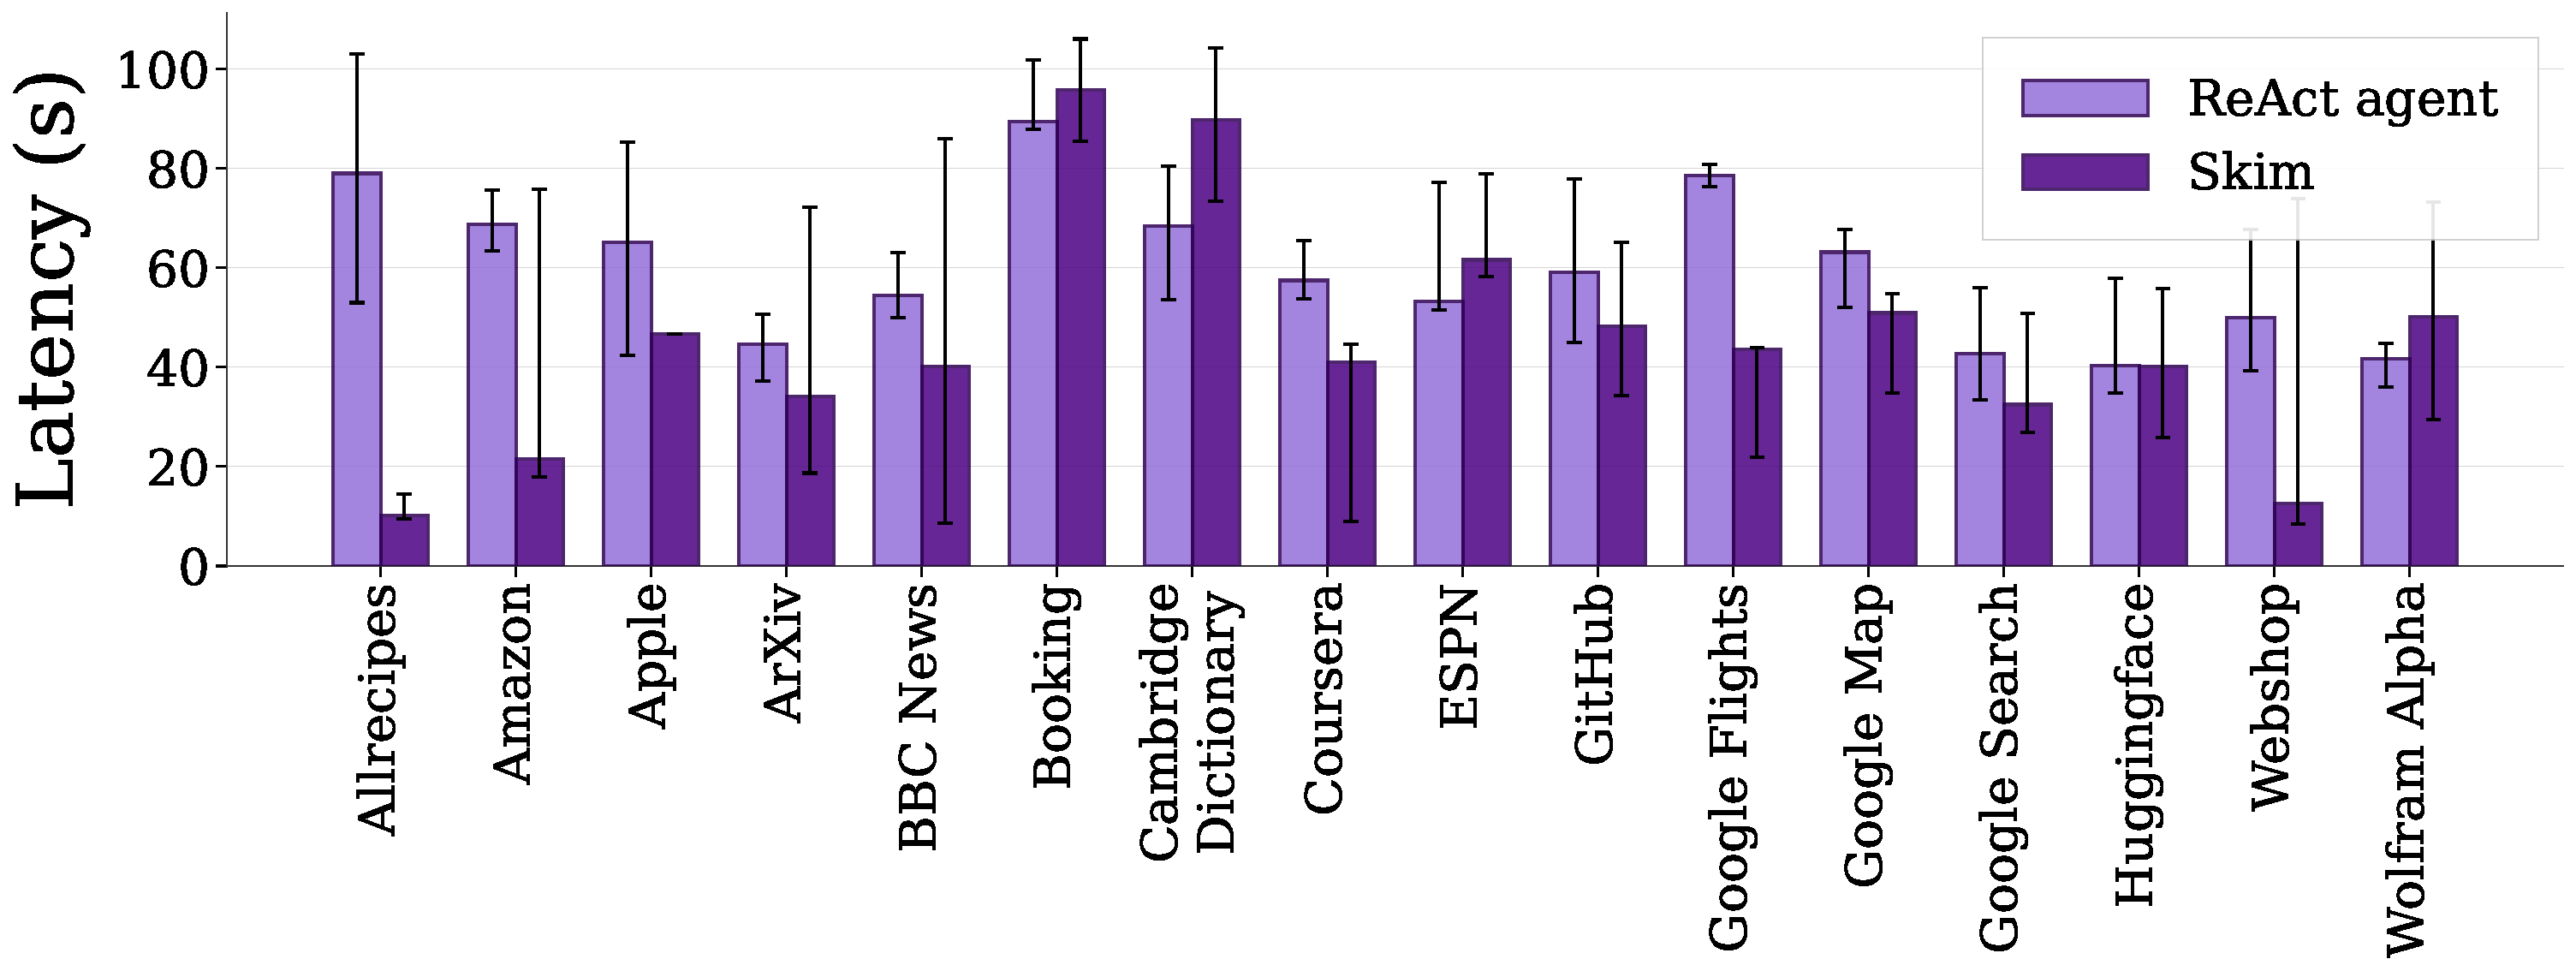
\includegraphics[width=0.9\columnwidth]{figures/latency_successful_breakdown_by_task_cdf.pdf}
    \tightcaption{Median end-to-end latency by website; error bars show 25th/75th percentiles. }
    \label{fig:eval-latency-breakdown-by-task}
\end{figure}

\para{Per-site speedups.}
Figure~\ref{fig:eval-latency-breakdown-by-task} reports median end-to-end latency across websites with heterogeneous retrieval and interaction structure. \sys{} achieves the largest speedups on sites whose workflows are dominated by structured search, filtering, and retrieval over stable page schemas. In these settings, speculative execution collapses multi-step browser interaction into direct URL synthesis followed by lightweight extraction over cleaned HTML, bypassing most of the iterative ReAct loop and avoiding many sequential browser actions and frontier-model inference calls. These gains are not tied to any single benchmark or domain; they emerge whenever a site exposes reusable navigation conventions and answer-bearing content resolvable through direct retrieval.

Latency improvements diminish on sites where speculation more frequently triggers fallback. These cases generally arise when site structure is difficult to parameterize through stable templates alone -- heavily JavaScript-driven interfaces, aggressive bot-detection, multimodal content requiring visual reasoning, or search semantics highly sensitive to exact query phrasing -- making direct retrieval less reliable and increasing verification failure and cascade. A small number of tasks also show speculative execution slightly increasing latency relative to the baseline, primarily when the warm start provides little useful navigational progress or when nondeterminism in LLM-based agent execution causes the baseline agent to converge unusually quickly. Even then, the overhead from failed speculation remains small relative to the cost of full browser-agent execution.

\para{Decomposing the savings gap.}
Two structural factors gap our savings from the hand-engineered ceiling. First, \sys pays a generalization tax of ~5-6s per task for routing, URL synthesis, and capability prediction. Second, only 12.6-45.3\% complete on the fast path; the rest cascade with warm-started ReAct, which captures most of the remaining gain through prefix-sharing rather than direct speculation success.
\begin{figure}[t]
    \centering
    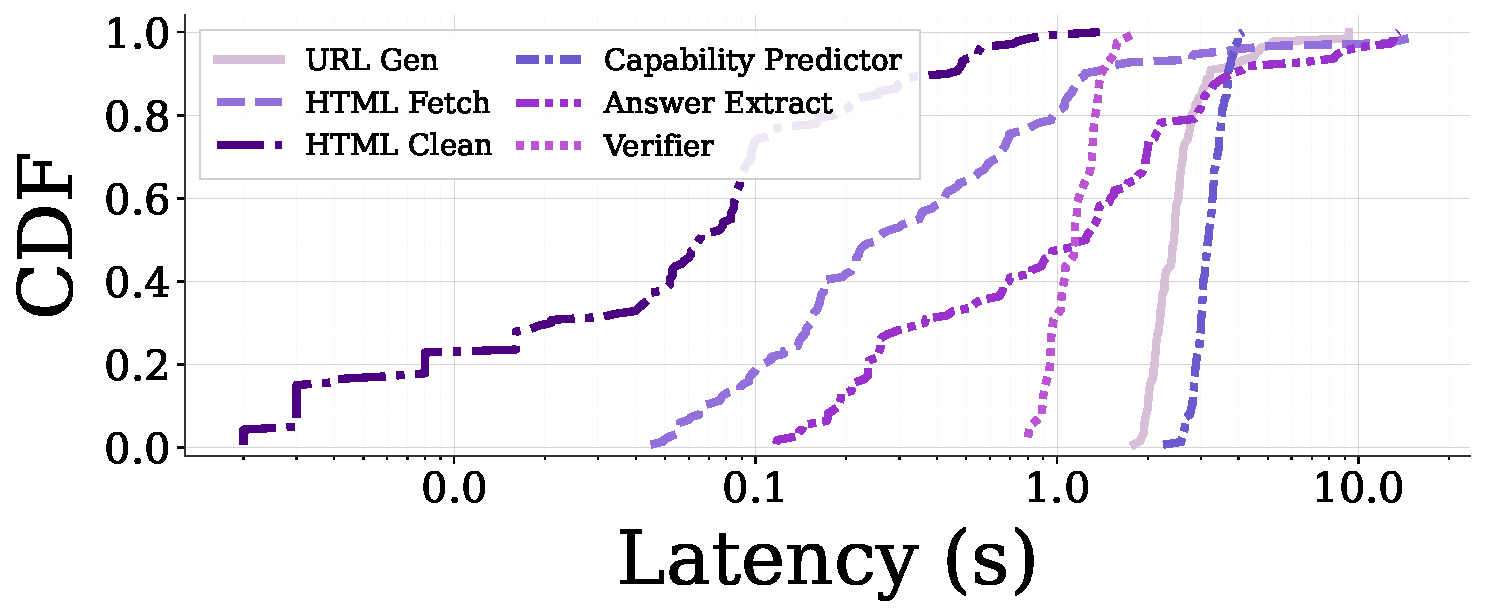
\includegraphics[width=0.9\columnwidth]{figures/ours_component_breakdown.pdf}
    \tightcaption{Per-task latency breakdown}
    \label{fig:eval-latency-breakdown}
\end{figure}

\para{Impact of warm starts.}
Figures~\ref{fig:warm-start-webvoyager-savings} and
\ref{fig:warm-start-agentoccam-savings} compare fallback latency
under warm- vs cold-started ReAct execution. Warm starts reduce fallback latency by
seeding the downstream agent with the URL reached during
speculative execution instead of restarting from the homepage.
Even when the fast path fails, it often resolves substantial
parts of the trajectory (search, filtering, pagination, query
construction), so fallback resembles local recovery from a
near-correct state rather than exploratory browsing from
scratch. The latency distributions show that this substantially
compresses the tail of expensive fallback trajectories across
both agents. This reflects the prefix-sharing property:
incorrect speculative trajectories remain close enough to the
correct path that ReAct recovers with little additional
exploration, allowing \sys{} to preserve latency gains even on
cascade.


\subsection{Detailed Analysis}

\para{Latency breakdown.}
We decompose per-task latency across system components to identify where time is spent along the speculative execution path. Figure~\ref{fig:eval-latency-breakdown} reports stage-level wall-clock latency for fast-path-completing tasks across six stages: routing and capability prediction, URL synthesis, HTTP fetch, HTML cleaning, lightweight extraction, and verification. The dominant costs arise not from web access itself, but from the lightweight semantic stages responsible for interpreting and parameterizing tasks: routing and capability prediction take $\sim$3s per task, and URL synthesis another $\sim$2--3s for most queries (with a small long tail reaching $\sim$9s). By contrast, the systems-oriented stages are extremely cheap: HTTP fetches typically complete within 100--300ms, and HTML cleaning is usually below 100ms. This highlights a central property of read-only web tasks: once the correct destination URL is known, retrieving and condensing the relevant content is inexpensive relative to discovering that URL through exploratory browser interaction.

Extraction latency exhibits the largest variance: simple schema-constrained retrievals complete in well under a second, while harder synthesis-style tasks occasionally require 8--14s of local-model reasoning. Verification adds only $\sim$1s of overhead, preserving the design goal that correctness checking remain cheaper than the speculative execution it validates. For cascaded tasks, the full ReAct loop dominates tail latency, but failed fast paths frequently still preserve useful navigational progress through warm-start URLs, allowing the downstream agent to resume near the relevant destination page rather than restarting from the homepage. Per-task cost follows the same asymmetry: fast-path tasks are dominated by inexpensive local-model inference and HTTP execution, while cascaded tasks inherit the frontier-model cost profile of full browser-agent execution.

\begin{figure}[t]
    \centering
    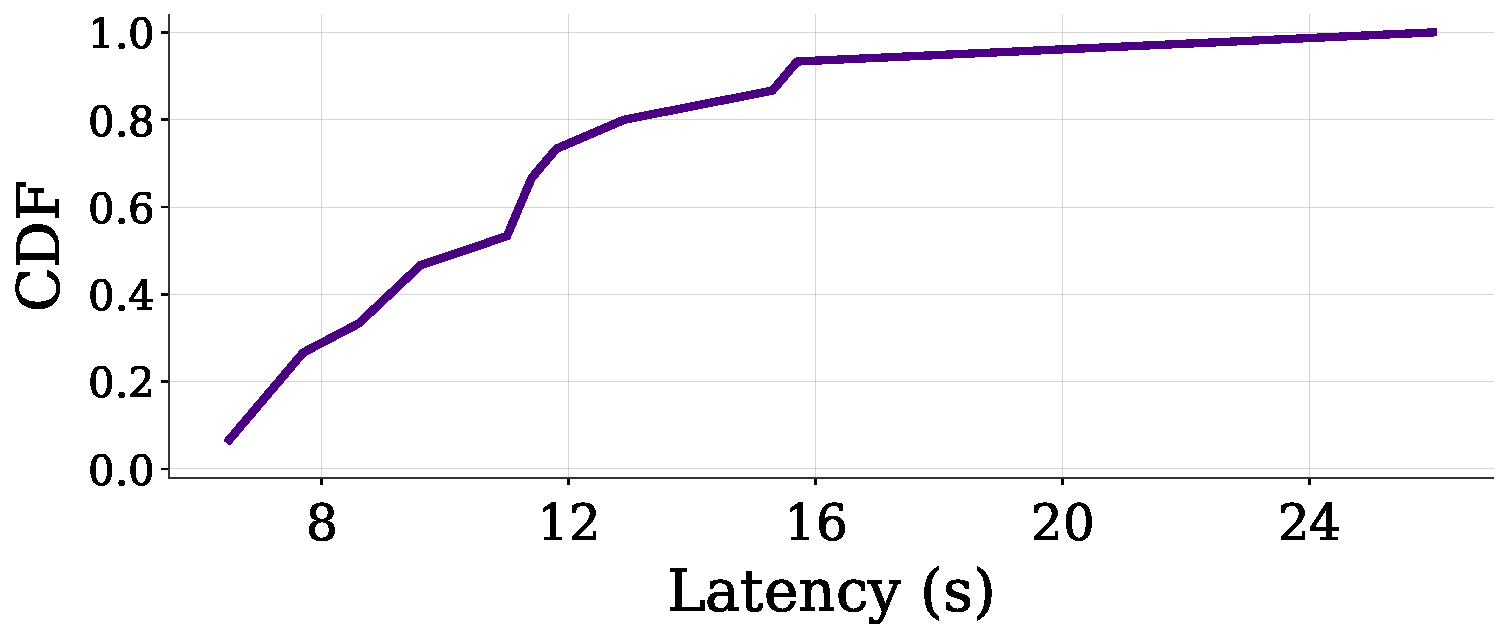
\includegraphics[width=0.9\columnwidth]{figures/offline_probing_latencies_cdf.pdf}
    \tightcaption{Offline profiling latency per site. }
    \label{fig:offline-profiling-cdf}
\end{figure}


\para{Verification cost vs. quality.} The verifier must satisfy two goals: it must remain cheap enough that verification does not erase the fast path's savings, while being conservative enough that incorrect speculative answers rarely commit. We therefore explicitly bias the verifier toward rejection and aggressive cascade rather than risking false accepts: borderline or weakly-supported speculative outputs are escalated to heavier execution tiers instead of being committed directly.

We compare \sys's lightweight verifier against a frontier-model verifier that scores candidate answers against the full DOM. The lightweight verifier is 11.5$\times$ cheaper per call while achieving 82.0\% precision and 86.2\% recall (F1 = 0.84, accuracy = 86.9\%). Reliability is highest on sites with structured, schema-friendly outputs and lower on sites with heavier client-side rendering or looser semantics; importantly, these are also the sites where speculative execution more frequently triggers fallback, so verifier uncertainty naturally translates into cascade rather than silently committed errors.

\para{Offline profiling pipeline.}
Figure~\ref{fig:offline-profiling-cdf} shows the one-time cost
of offline profiling. Profiling completes within 10s for
${\sim}40$\% of sites and within 12s for ${\sim}60$\%, with a
small tail toward 16s on structurally complex sites requiring
browser escalation, dynamic rendering, or bot-detection
handling. The cost stays this low because the profiler captures
the small set of URL templates and answer schemas that cover
common-case tasks rather than enumerating every page or query
the site supports; tasks that fall outside profiled patterns
are detected at match time and routed to the ReAct fallback, so
coverage gaps cost nothing in correctness. The cost is amortized
across all future tasks on the site and does not contribute to
online query latency. Profiles are continuously validated
through schema and content-consistency checks at runtime; stale
profiles are regenerated when structural drift is detected.



% \para{Comparison with stateless retrieval pipelines.}
% Production retrieval-augmented assistants (Perplexity, Gemini
% grounded search, ChatGPT browsing) operate as stateless retrieval
% pipelines: they issue a query to a search API, fetch the top-ranked
% results, and synthesize an answer. This pattern is efficient on
% tasks whose answers are surfaced by search-engine indices but is
% structurally bounded by index coverage. Our SearXNG+GPT-4o baseline,
% a representative single-shot instance of this pattern, succeeds on
% $S_{sr}$\% of WebVoyager tasks at \$$C_{sr}$ per task. It fails on
% the regime stateless retrieval is structurally limited on:
% authenticated or session-bound pages, multi-step trajectories whose
% intermediate states are not search-indexed, and freshly-published
% or niche content beyond search-engine coverage. \sys reaches
% stateless-retrieval cost on its fast path while preserving full
% ReAct's coverage on the cascaded tail, occupying a different point
% in the cost-coverage tradeoff than either pure approach. \todo{Need to get these stateless retrieval numbers}



